\chapter{Contexte général du projet}
\label{chap:Contexte général du projet}



Ce chapitre situe mon projet de fin d’études dans son environnement organisationnel et contextuel. Il commence par une présentation de l’organisme d’accueil, SQLI Maroc. Ensuite, il détaille la problématique ayant conduit à la réalisation de ce projet ainsi que les objectifs visés. Enfin, la méthodologie adoptée pour mener à bien le projet est abordée.

\newpage


\section{Présentation de l’entreprise d’accueil SQLI}

Cette section initiale met en lumière le Groupe SQLI en mettant l’accent sur ses activités clés, son
chiffre d’affaires ainsi que ses clients. Ensuite, l'accent sera mis sur SQLI Maroc, en mettant en avant ses valeurs fondamentales.

\subsection{Groupe SQLI}

\begin{figure}[h]
    \centering
    
\includegraphics[scale=0.7]{Logos/SQLI_LOGO.png} % Replace with the actual filename of the IBM logo image
    \caption{Logo de SQLI \cite{SQLI}}
    \label{fig:LogoSQLI}
\end{figure}

SQLI est une entreprise européenne de services numériques fondée en 1990 par Jean Rouveyrol et Alain Lefebvre. Elle se spécialise dans la conception, le développement et le déploiement de solutions digitales
visant à créer des expériences unifiées \cite{SQLI}. Avec un effectif de 2400 collaborateurs répartis dans 13 pays,
SQLI bénéficie d’une présence internationale solide.

Le succès de SQLI Digital Experience repose sur des valeurs fondamentales telles que la créativité, l'engagement et l'audace visionnaire. Ces valeurs imprègnent chaque aspect de l'entreprise, permettant de repousser les frontières de l'innovation et de concevoir des expériences digitales uniques et captivantes. \cite{valeurSQLI}

\subsubsection{Activités du groupe}

Le groupe SQLI propose une gamme étendue de services pour accompagner les entreprises dans leur transformation numérique. Il inclut l'e-commerce, créant et optimisant des plateformes de vente en ligne performantes. Il offre également des plateformes d'expérience, conçues pour offrir des interactions utilisateur exceptionnelles. En matière de technologie et de transformation, il aide les entreprises à moderniser leurs infrastructures et leurs processus. Ses services de data et insights permettent d'exploiter les données de manière stratégique, tandis que son expertise en marketing digital et design améliore la visibilité et l'attrait des marques. Enfin, son conseil digital guide les entreprises dans l'élaboration et la mise en œuvre de leur stratégie numérique globale, assurant ainsi une transformation digitale réussie. \cite{SQLI}

\subsubsection{Chiffres Clés du groupe}

Les chiffres clés suivants présentent la situation actuelle de SQLI :

\begin{itemize}
    \item[$\bullet$] Fort de 33 ans d’expérience et d’innovation, SQLI fonde son développement sur une expertise technologique de pointe et une politique de veille intensive.
    \item[$\bullet$] SQLI emploie plus de 2400 collaborateurs répartis dans 13 pays, notamment la France, l'Angleterre, la Suède, les Pays-Bas, l'Espagne, l'Allemagne, la Belgique, le Luxembourg, la Suisse et le Maroc.
    \item[$\bullet$] En 2022, le groupe SQLI a atteint un chiffre d’affaires de 251,2 millions de dollars. Ce succès est le résultat d'une offre bien alignée sur les attentes du marché et d'une reprise progressive de la demande de services informatiques.
    \vspace{0.5cm}
\end{itemize}

\begin{figure}[H]
    \centering
    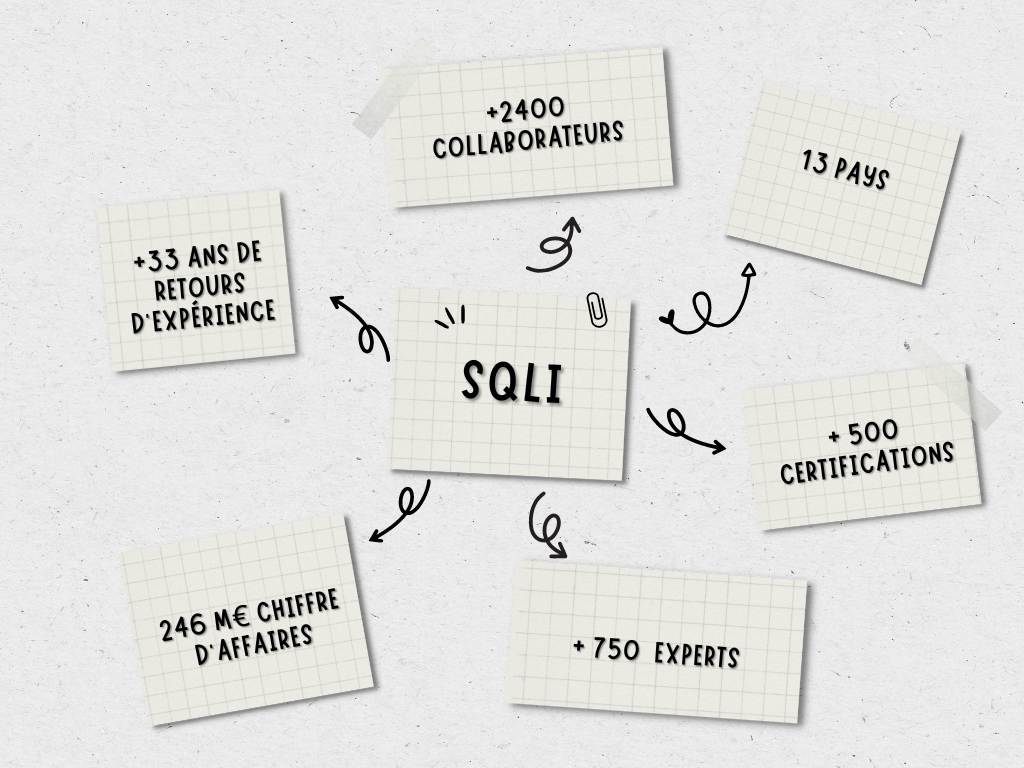
\includegraphics[width=10cm]{Figures/cle chiffre.png} % Replace with the actual filename of the IBM logo image
    \caption{Chiffre Clés de SQLI}
\end{figure}

\subsubsection{Clients du groupe}

SQLI collabore avec une vaste gamme de clients provenant de divers secteurs, y compris l'automobile, la distribution, la banque et l'assurance, le luxe et la mode, la santé, l'industrie et l'énergie, ainsi que les télécommunications. Les grandes entreprises internationales et les organisations locales font appel à SQLI pour ses solutions digitales innovantes, allant de l'optimisation des plateformes d'e-commerce à la transformation numérique des services financiers, en passant par la création d'expériences utilisateur uniques pour les marques de luxe et la digitalisation des processus industriels. Grâce à sa capacité à répondre aux besoins spécifiques de chaque secteur, SQLI bâtit des partenariats solides et durables avec ses clients (\textit{Figure~\ref{fig:client}})

\begin{figure}[H]
    \centering
    
\includegraphics[width=15cm]{Figures/sqli partenaire .png} % Replace with the actual filename of the IBM logo image
    \caption{Clients du SQLI \cite{SQLI}}
    \label{fig:client}
\end{figure}


\subsection{SQLI Maroc}

SQLI Maroc, créée en 2003 à Rabat par Eric Chanal, représente le centre de Delivery et d'Innovation du Groupe SQLI. Bénéficiant d'une solide expertise et d'une grande expérience, l'entreprise est présente sur trois sites stratégiques : Rabat, où j'ai eu l'opportunité d'effectuer mon stage PFE, Oujda et Casablanca. Le tableau \textit{\ref{tab:fiche}} représente sa fiche technique:



% l'ajoute de titre de tableau avec space between titre de tab et le tab
% \captionsetup{type=table}

% \vspace{0.3cm}
% tab
\begin{center}
    \captionsetup{type=table}
    \vspace{0.3cm}
    \begin{tabularx}{17cm}{|X|X|}
      \hline
     \textbf{Dénomination sociale}  & \textbf{SQLI Digital Experience} \\
      \hline
     {Année de fondation} & 2003  \\
      \hline
      {Fondateur} & Eric Chanal  \\
      \hline
     {Siège social} & Rabat, Maroc\\
     \hline  
     {Activité} & Conseil en systèmes et logiciels informatiques.\\
      \hline  
     {Effectif des employés} & Plus de 900 collaborateurs.\\
      \hline
     {Sites d'implantation} & Rabat, Oujda et Casablanca.\\
      \hline
    \end{tabularx}
    \captionof{table}{Fiche technique de SQLI Maroc}
    \label{tab:fiche}
    \end{center}
    

  SQLI Maroc comprend principalement deux structures essentielles, présentées dans la \textit{Figure~\ref{fig:departement}}, à savoir :

\begin{enumerate}
    \item \textbf{SQLI WAX INTERRACTIVE} : accompagne les clients dans leur transition vers la digitalisation afin de renforcer leur positionnement sur le marché. Cette entité intervient principalement sur le plan stratégique en collaborant étroitement avec les clients.
     \item \textbf{SQLI ENTREPRISE} : est chargée de la mise en œuvre des systèmes d'information pour les clients. Elle se compose de plusieurs Business Units spécialisées dans différents domaines :
\begin{itemize}

    \item [$\bullet$]\textbf{E-commerce/ JAVA EE} : Se focalise sur la création et la mise en place de sites de e-commerce ainsi que sur le développement d’applications utilisant la technologie Java EE.
    \item [$\bullet$]\textbf{Mobile/Front} : Se spécialise dans le développement d’applications mobiles et l’interface utilisateur (front-end) pour les clients.
    \item [$\bullet$]\textbf{Microsoft} : S'occupe de la réalisation d’applications basées sur les technologies Microsoft.
    \item [$\bullet$]\textbf{Agency} : Joue un rôle transversal en assurant la conception de l’interface utilisateur (front-end) pour toutes les autres Business Units.
    \item [$\bullet$]\textbf{Delivery} : Se charge de la gestion des livraisons et des recettes auprès des clients.
\end{itemize}
\end{enumerate}
\vspace{0.5cm}
\begin{figure}[H]  
  \centering  
  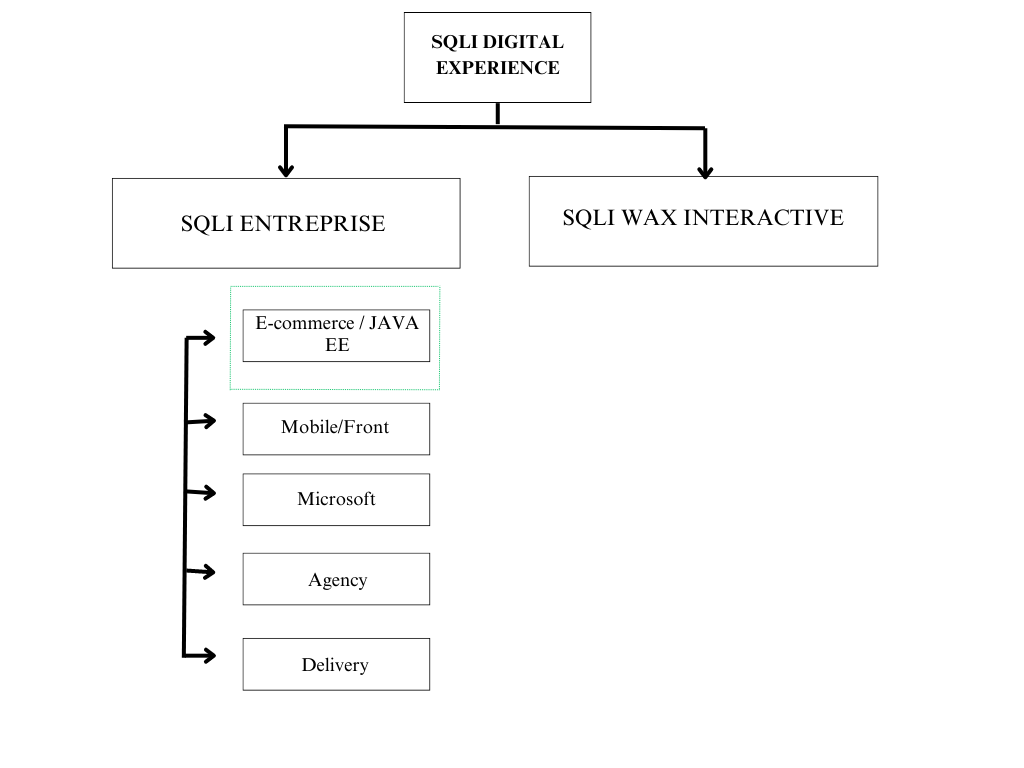
\includegraphics[width=14cm]{Figures/departement.png}
  \caption{Départements de SQLI}
  \label{fig:departement}
\end{figure}


Mon stage de fin d'études s'est déroulé dans le département Java JEE, qui regroupe plusieurs projets destinés à des grandes entreprises clientes.


\section{Présentation du projet}

\subsection{Cadre du projet et problématique}

Dans le cadre d'un projet e-commerce pour un client de luxe, l'objectif est d'améliorer et d'optimiser sa plateforme actuelle. Il est indispensable de mettre à jour régulièrement cette plateforme, qui joue un rôle crucial dans les activités commerciales en ligne du client, afin de maintenir sa compétitivité et de répondre aux exigences du marché.

Pour cette amélioration, le travail inclut la correction de divers bugs qui affectent la performance et la fiabilité du système. La résolution de ces bugs est cruciale pour garantir une expérience utilisateur fluide et sans interruptions.

En parallèle, l'intégration de nouvelles fonctionnalités est nécessaire pour enrichir l'offre de la plateforme. L'un des changements majeurs est l'intégration de la méthode de paiement Payconiq, destinée spécifiquement au marché belge. Différents défis se posent lors de cette intégration, tels que la compatibilité avec l'architecture existante, la gestion des dépendances et l'assurance que cette nouvelle fonctionnalité ne provoque pas de régressions ou de nouveaux bugs.

L'enjeu majeur consiste donc à corriger les bugs existants tout en intégrant Payconiq de manière efficace, en maintenant la stabilité et la performance globale de la plateforme.

 \subsection{Objectifs du projet}

 Dans le cadre de ce projet, je participerai activement aux diverses activités de l'équipe, contribuant à la fois au développement des fonctionnalités demandées par le client et à l'amélioration continue du système. Les objectifs spécifiques de mon intervention sont les suivants :

 \begin{itemize}
    \item[$\bullet$] \textbf{Intégrer un nouveau mode de paiement, Payconiq, pour le marché belge } 
    
    Analyser et comprendre l'architecture existante pour intégrer Payconiq, tout en gérant les dépendances et en garantissant la compatibilité avec les autres modules de la plateforme, conformément aux spécificités techniques du marché belge. Cela inclut la configuration, le développement, et des tests rigoureux pour garantir une intégration fluide dans les différents flux de paiement existants.

    \item[$\bullet$] \textbf{Assurer les livraisons dans différents environnements (DEV, INTx, UAT, PRD) } 
    
    Garantir le bon fonctionnement du code dans chacun de ces environnements, conformément aux exigences de stabilité et de performance. Cela comprend des tests approfondis pour s'assurer que les nouvelles fonctionnalités et intégrations sont stables et opérationnelles avant la mise en production.

    \item[$\bullet$] \textbf{Respecter les meilleures pratiques, les normes, et l'architecture du projet } 
    
    Assurer la cohérence du code et la stabilité du projet en adhérant aux normes et pratiques de développement établies. Cela inclut le respect des principes d'architecture définis, l'application des bonnes pratiques de codage, et la proposition de solutions conformes aux standards en vigueur au sein de l'équipe.

    \item[$\bullet$] \textbf{Analyser et corriger les bugs détectés }
    
    Assurer la maintenance corrective du système en identifiant, analysant, et résolvant les bugs remontés par les équipes du projet ou découverts lors des tests, afin de minimiser leur impact sur le fonctionnement global de la plateforme.

\end{itemize}

 %%%%%%%%%%%%%%%%%%%% SECTION 4 %%%%%%%%%%%%%%%%%%%%%%%
\section{Conduite de projet}

\subsection{Présentation des Équipes du Projet}

Après ma période de formation, j’ai intégré une première équipe en tant que stagiaire backend. Cette équipe était responsable des aspects liés à la recherche, aux lunettes et à la mode pour le projet Chanel. À mon arrivée, l'équipe se concentrait sur le Plan 99.5, visant à analyser les bugs, nettoyer les logs, corriger les erreurs et refactoriser le code. La structure de cette équipe est illustrée dans la \textit{Figure~\ref{fig:structure_seasonal_event}}.

Souhaitant approfondir mes compétences dans des domaines complémentaires, j'ai ensuite rejoint une autre équipe, chargée de l’intégration des nouvelles méthodes de paiement pour les différents marchés du client. La structure de cette équipe est illustrée dans la \textit{Figure~\ref{fig:structure_payment}}.

Ces deux équipes font partie d'un projet plus vaste comprenant 15 équipes fonctionnelles différentes. Chaque équipe est composée d'un Scrum Master, d'un expert technique, d'un Product Owner, d'un développeur frontend et de deux responsables qualité, favorisant ainsi le développement d'une solution robuste et performante.

\begin{center}
    \centering
    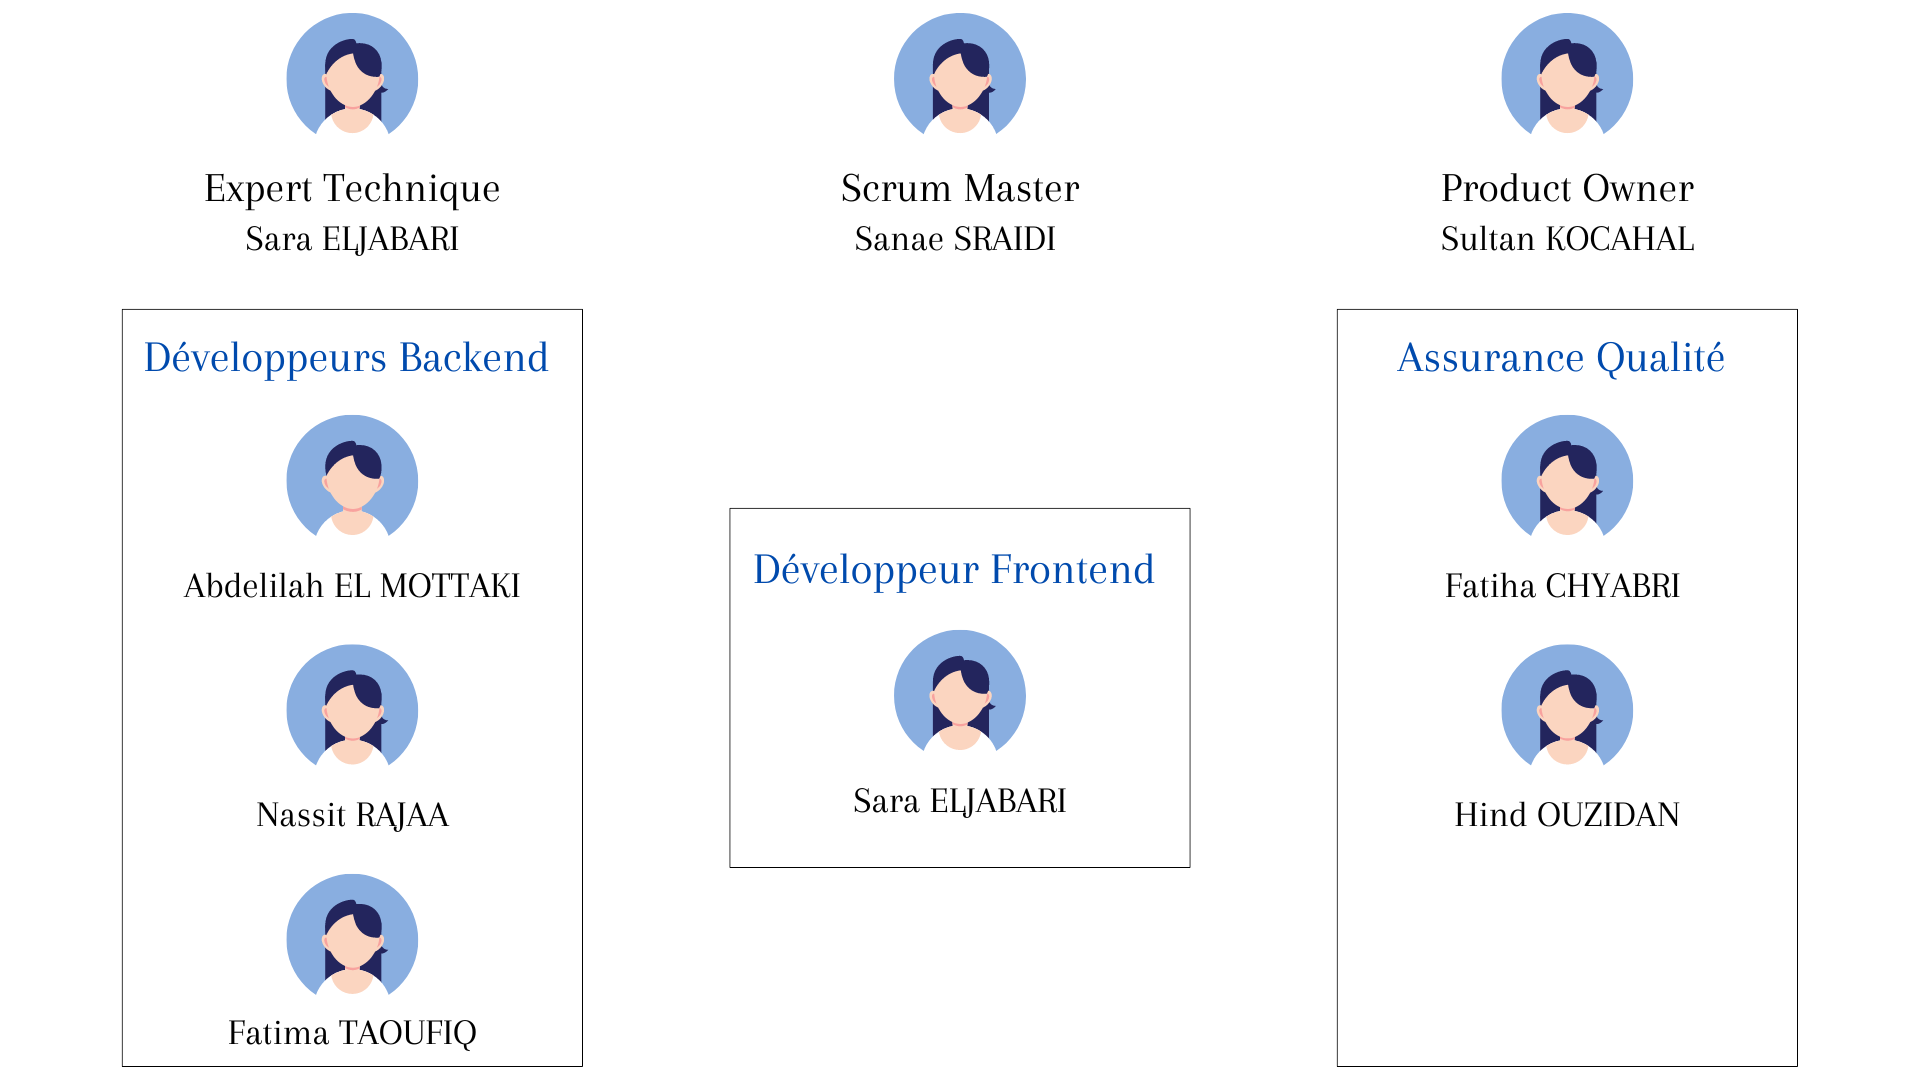
\includegraphics[width=19cm]{Figures/Seasonal Event Team.png}
    \captionof{figure}{Structure de l'équipe Seasonal Event}
    \label{fig:structure_seasonal_event}
\end{center}

\begin{center}
    \centering
    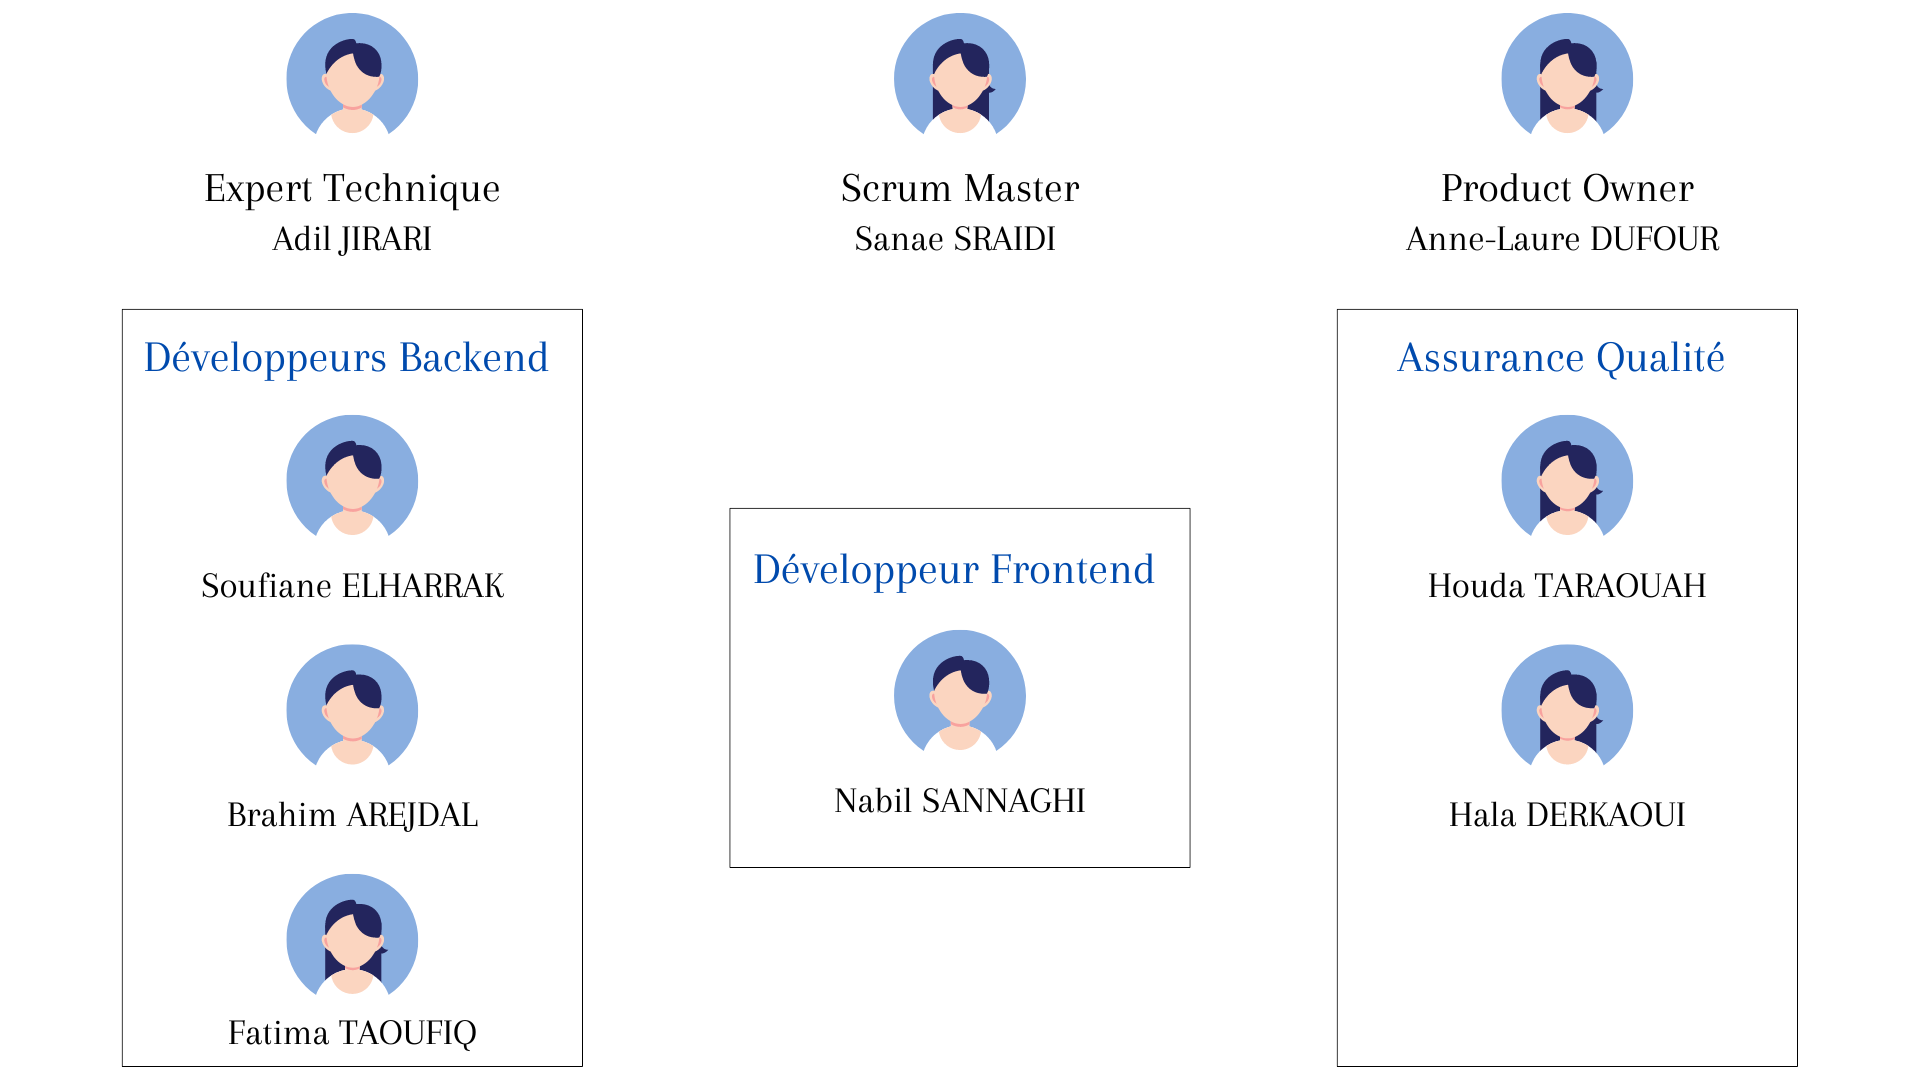
\includegraphics[width=19cm]{Figures/Cart Checkout & Payment.png}
    \captionof{figure}{Structure de l'équipe Cart Checkout \& Payment}
    \label{fig:structure_payment}
\end{center}


\subsection{Méthodologie de travail : Scrum}

Pour assurer une collaboration efficace au sein de l'équipe, nous avons opté pour la méthodologie Scrum, qui se caractérise par une approche itérative et incrémentale. Scrum nous permet de diviser le travail en sprints, des cycles de développement courts et cadencés, généralement de deux à quatre semaines. À la fin de chaque sprint, une version potentiellement livrable du produit est présentée, ce qui favorise la flexibilité et l'adaptation aux changements. Grâce à cette méthode, nous pouvons rester réactifs et ajuster rapidement notre travail en fonction des évolutions des besoins métiers. En intégrant les retours d'expérience du client à chaque itération, nous assurons une satisfaction optimale de ses attentes. Les rôles bien définis, tels que le Scrum Master, le Product Owner, et l'équipe de développement, garantissent une communication claire et une responsabilité partagée. Cette approche nous permet d'être efficaces tout en maintenant un rythme de travail soutenu et structuré.


\textbf{\textbullet \textit{Planification du sprint (sprint planning)}}

Avant de débuter chaque sprint, nous tenons une réunion de Sprint Planning. Cette réunion a pour objectif de définir les tâches prioritaires à accomplir au cours du sprint à venir. L'équipe, en collaboration avec le Product Owner, examine le backlog du produit pour identifier les éléments les plus critiques à traiter. Durant cette session, nous discutons des exigences, des objectifs du sprint, et nous évaluons la charge de travail nécessaire pour chaque tâche. Cette planification permet à l'équipe de se concentrer sur un ensemble de fonctionnalités claires et réalisables, tout en s'assurant que les ressources sont allouées de manière optimale. Ainsi, chacun sait précisément sur quoi se concentrer, ce qui contribue à une exécution efficace et coordonnée du sprint.

\textbf{\textbullet \textit{Mêlée quotidienne (Daily Meeting)}}

Chaque jour, nous tenons une réunion appelée Daily Meeting, d'une durée de 15 minutes chaque matin. Lors de cette réunion, chaque membre de l'équipe partage ce qu'il a accompli la veille, ce qu'il prévoit de faire aujourd'hui, et signale s'il rencontre des problèmes ou des blocages. Cette réunion permet à l'équipe de rester synchronisée et d'identifier rapidement les obstacles éventuels, favorisant ainsi une meilleure collaboration et une résolution rapide des problèmes.

\textbf{\textbullet \textit{Revue de sprint (Sprint Review) }}

La revue de sprint se tient à la fin de chaque sprint pour présenter et évaluer les fonctionnalités développées. L'équipe démontre le travail accompli aux parties prenantes, recueille leurs retours et discute des ajustements nécessaires. Ce moment est crucial pour valider les résultats, s'assurer qu'ils répondent aux attentes et planifier les prochaines étapes en fonction des feedbacks reçus.

\textbf{\textbullet \textit{Rétrospective de sprint }}

À la fin de chaque sprint, nous tenons une rétrospective de sprint, un moment privilégié pour discuter des succès et des aspects à améliorer dans notre travail. Pour détendre l'atmosphère et réduire le stress, nous intégrons également de petits jeux qui permettent de sortir de la routine, de mieux connaître les membres de l'équipe, et de renforcer notre cohésion. Ces activités, combinées à des discussions constructives, nous aident à identifier les points à optimiser et à faire évoluer nos pratiques de manière continue.

\textbf{\textbullet \textit{Préparation du backlog (Backlog Refinement) }}

Nous tenons régulièrement des réunions de préparation du backlog, également appelées sessions d'affinement du backlog. Lors de ces réunions, l'équipe Scrum se réunit pour examiner et ajuster les éléments du backlog du produit. Nous clarifions les exigences, estimons les efforts nécessaires pour chaque tâche, et réorganisons les priorités en fonction des retours des parties prenantes et des évolutions du projet. Cette réunion est essentielle pour maintenir le backlog bien structuré et aligné avec les objectifs du projet, ce qui facilite une planification plus efficace des sprints et assure une gestion optimale des priorités.


\subsection{Capitalisation et suivi}

Pour assurer un suivi efficace du projet, l'équipe utilise des outils de gestion de projet tels que Azure DevOps et Confluence.

\textbf{\textbullet \textit{ Confluence}}

Confluence est utilisé pour la documentation et l'archivage des informations du projet, offrant une base de connaissances centralisée accessible à tous les membres de l'équipe. Cette plateforme permet de créer, organiser et maintenir des documents essentiels tels que les spécifications techniques, les guides de processus et les comptes rendus de réunions. En centralisant ces informations dans Confluence, nous facilitons la réutilisation des connaissances et assurons leur préservation au-delà de la durée du projet. Cette approche améliore la transparence, soutient la collaboration et garantit que les informations cruciales sont facilement accessibles pour toute l'équipe.

\begin{center}
    \centering
    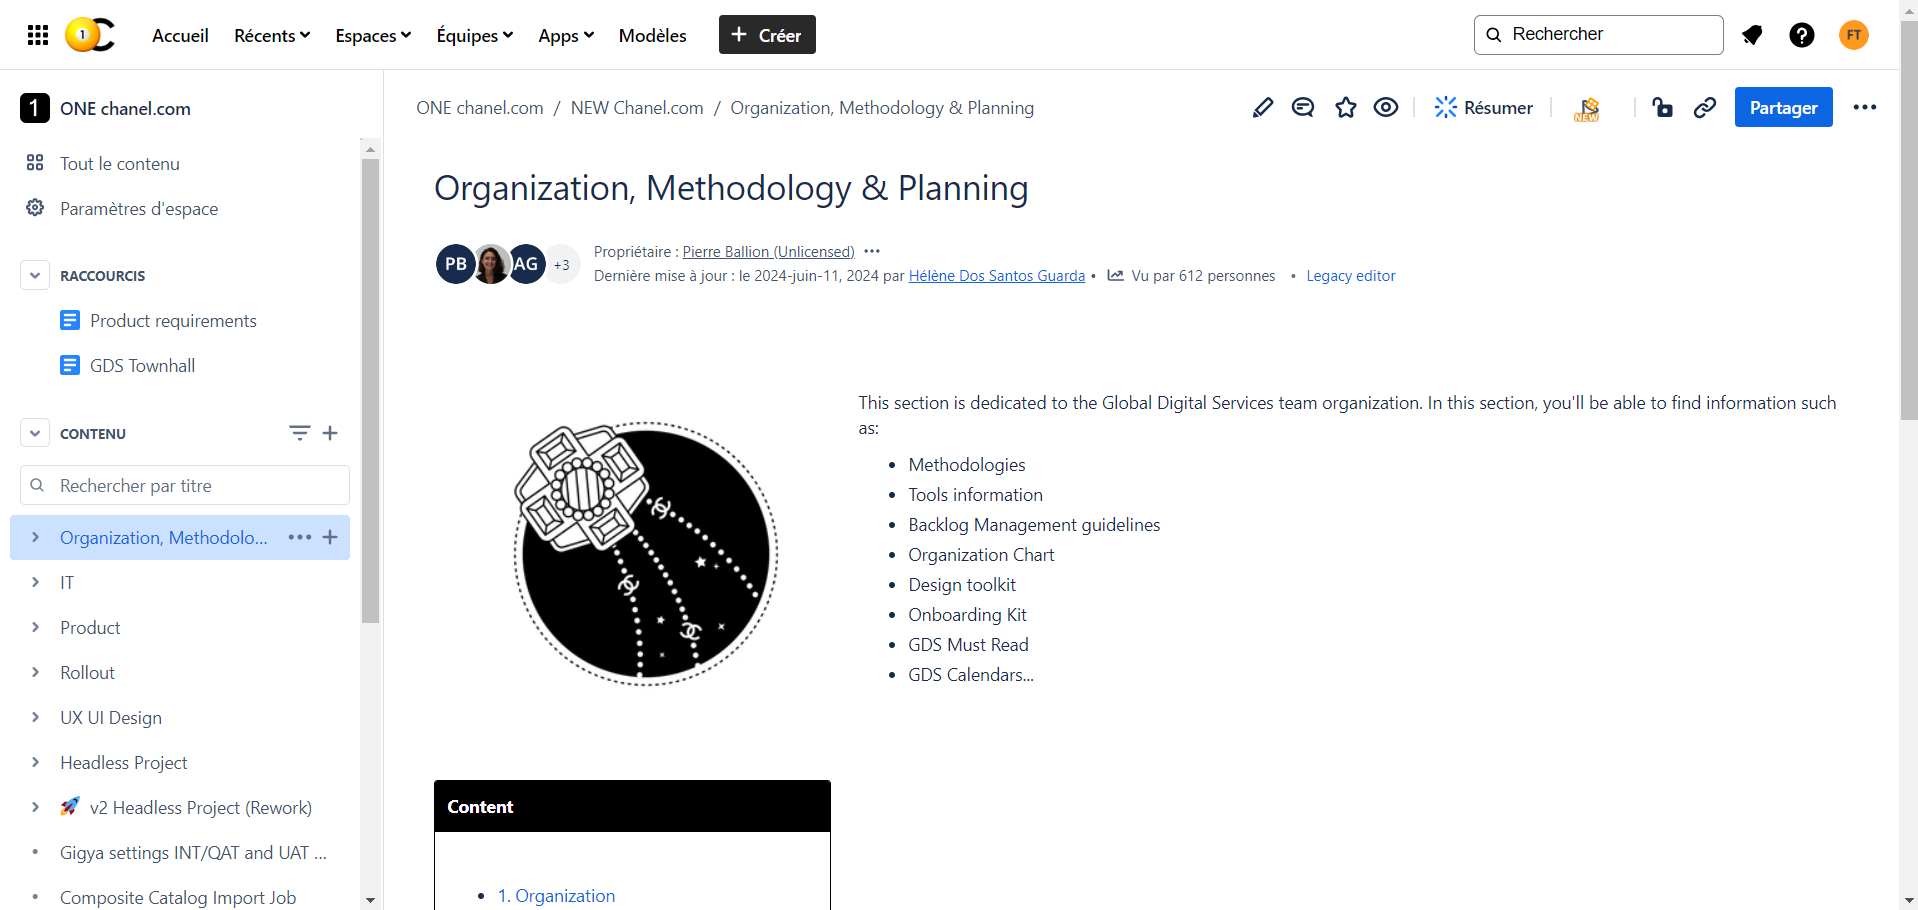
\includegraphics[width=19cm]{Figures/Confluence Documentation.png}
    \captionof{figure}{Page d’accueil de Confluence}
\end{center}


\textbf{\textbullet \textit{Azure DevOps}}

Azure DevOps nous permet de gérer efficacement les tâches à réaliser et de suivre en temps réel l'avancement de chaque membre de l'équipe. En plus de ces fonctionnalités de gestion de projet, Azure DevOps sert également de dépôt centralisé pour le code et les artefacts du projet, facilitant ainsi la collaboration et l'intégration continue.
\begin{center}
    \centering
    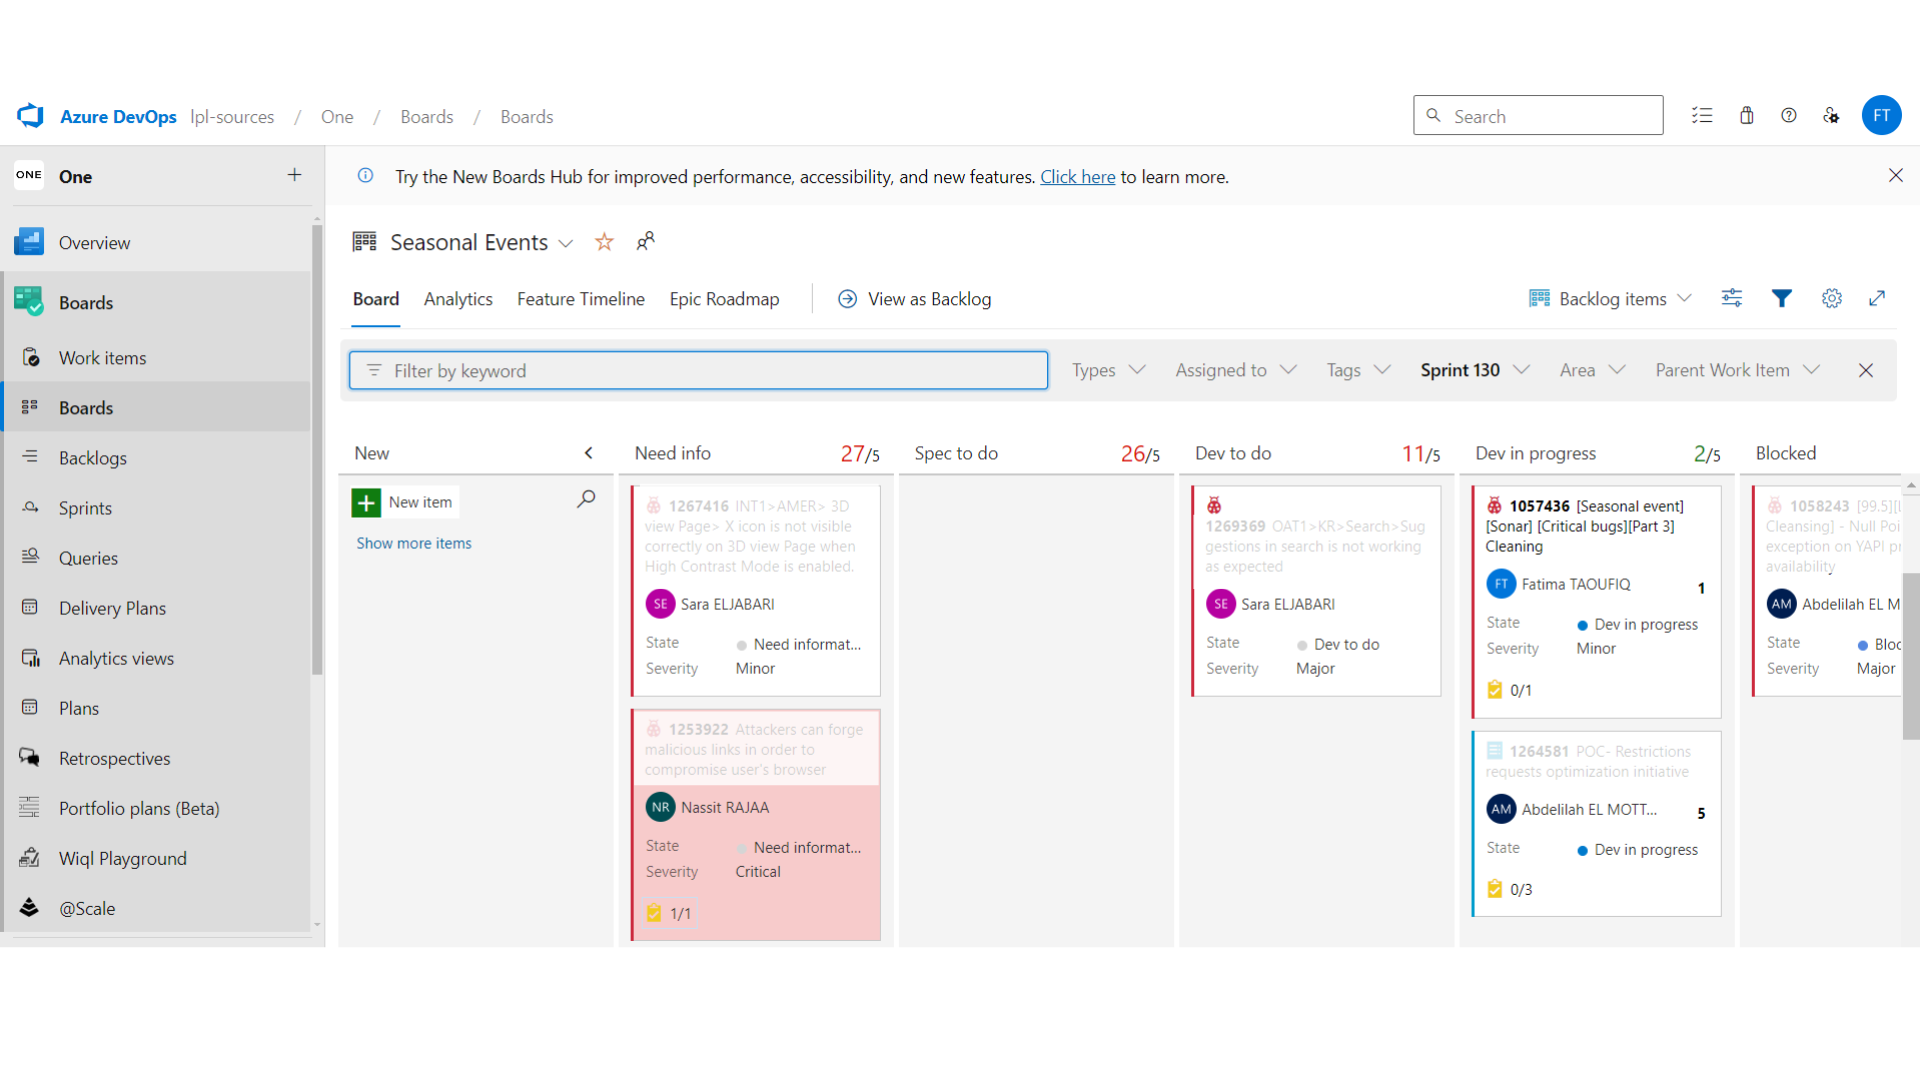
\includegraphics[width=18cm]{Figures/azure DevOps-tickets.png}
    \captionof{figure}{Backlog du projet sur Azure DevOps}
\end{center}

\textbf{\textbullet \textit{Microsoft Teams}}

Microsoft Teams est un outil essentiel pour la communication et la collaboration au sein du projet. Il nous permet de maintenir une communication fluide entre les managers, les chefs de projet, et les membres de l'équipe. Lorsqu'il est nécessaire de contacter quelqu'un pour obtenir des informations, poser des questions ou résoudre des problèmes, j'utilise Teams pour envoyer des messages instantanés, organiser des réunions virtuelles ou partager des documents. Cet outil facilite également la coordination des tâches et le suivi des progrès en centralisant les échanges et les informations pertinentes, ce qui contribue à une gestion de projet efficace et une meilleure intégration des membres de l'équipe.


\subsection{Planification du projet}

\subsubsection{Intégration}

Notre expérience a débuté par une journée d'intégration organisée par l'équipe RH, en collaboration avec les managers de chaque département. Cette journée a été l'occasion pour nous de découvrir en profondeur la structure de l'organisation, de comprendre les rôles et responsabilités de chacun, et de faire connaissance avec les collègues avec qui nous allions collaborer. Cette intégration nous a permis de nous familiariser rapidement avec notre environnement de travail et de tisser des liens avec les membres de l'équipe, facilitant ainsi notre adaptation et notre engagement au sein de l'entreprise.

\subsubsection{Formation}

La phase de formation, cruciale dans le cadre de notre stage, nous a permis d'acquérir les bases nécessaires pour réussir dans notre domaine. Cette formation, d'une durée de deux mois, a été animée par des professionnels expérimentés qui ont partagé avec nous leur savoir-faire et leur expertise. Grâce à ces sessions, nous avons pu renforcer nos compétences techniques et notre compréhension des bonnes pratiques du métier. Voici les principales formations qui ont constitué notre parcours :

\begin{center}
    \centering
    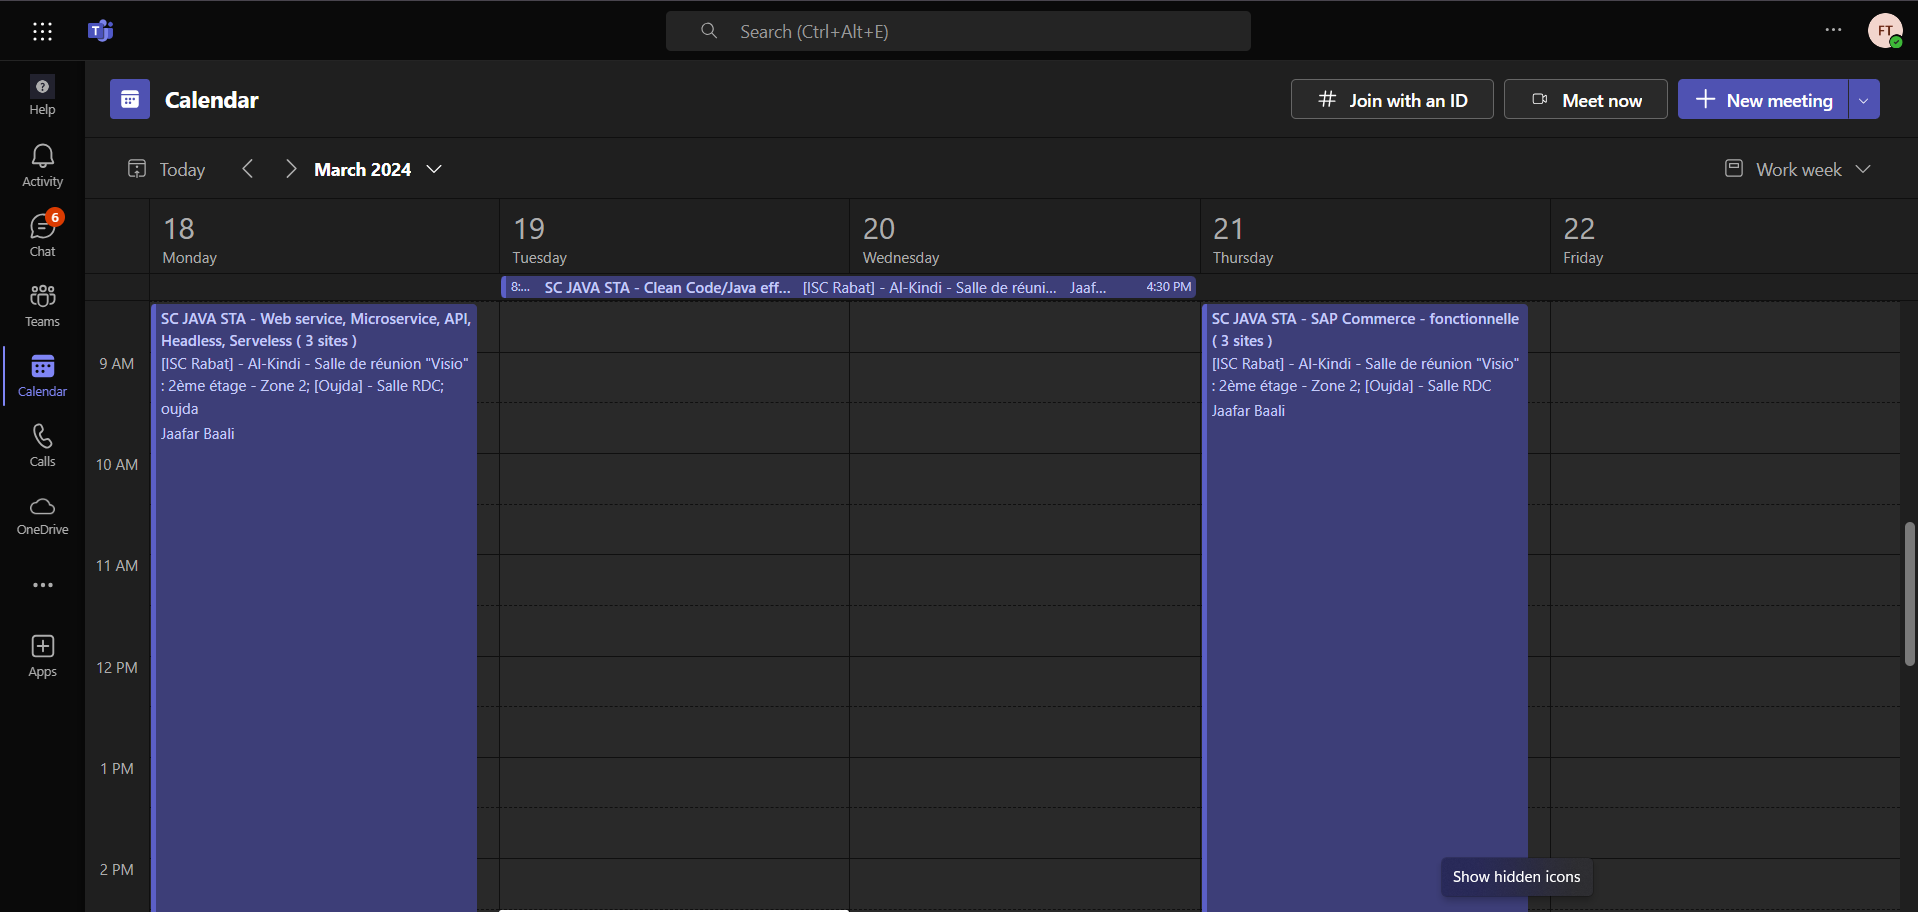
\includegraphics[width=19cm]{Figures/formation.png}
    \captionof{figure}{Clendrier des formations}
    \label{fig:structure_payment}
\end{center}
\begin{itemize}
    \item \textbf{\textit{Formations Spring :}}
    Durant cette formation, nous avons exploré les concepts fondamentaux du framework Spring, tels que l'inversion de contrôle (IoC) et Spring MVC. Ces notions clés ont été renforcées par des exercices pratiques pour mieux comprendre leur utilisation dans le développement d'applications Java.
    \item \textbf{\textit{Formations SAP Commerce (Hybris) :}}
    Pendant cette formation, nous avons commencé par installer la plateforme SAP Commerce. Nous avons ensuite exploré les aspects fonctionnels, comme l'utilisation des outils d'administration HAC, HMC, et des différents Cockpits. En parallèle, nous avons approfondi des sujets techniques, tels que la configuration de CronJobs et la gestion des workflows.
    \item  \textbf{\textit{Formations Clean Code :}}
    Cette formation, inspirée des principes de Robert C. Martin, nous a appris les bonnes pratiques pour écrire du code propre, lisible et maintenable. Nous avons appliqué ces concepts à travers des exercices pratiques, axés sur la structuration du code et les techniques de refactoring.
    \item \textbf{\textit{ Formations Software Craftsmanship :}}
    La formation en Software Craftsmanship s'est concentrée sur l'excellence technique et la qualité du code. Nous avons étudié des pratiques comme le pair programming, la revue de code, et l'écriture de tests automatisés, renforçant ainsi notre capacité à produire du code robuste et maintenable.
    \item \textbf{\textit{Formations ICD Skills \& Agilité :}}
    Cette formation nous a initiés aux compétences interpersonnelles essentielles et aux méthodes agiles. Nous avons étudié des méthodologies comme Scrum et Kanban, et nous avons mis en pratique des techniques de gestion de projet agile pour améliorer notre efficacité et notre adaptabilité en équipe.
\end{itemize}
\subsubsection{Intégration du projet}

J'ai été affecté au projet Chanel ONE en tant qu'ingénieur backend, avec pour mission principale l'intégration de la méthode de paiement Payconiq pour le marché belge. En plus de cette tâche, j'ai également travaillé sur la correction de bugs, en particulier ceux liés à Sonar, en mettant à profit ma solide connaissance de cet outil pour améliorer la qualité du code et réaliser les refactorings nécessaires. Mon intégration dans le projet a débuté par une phase de onboarding de 15 jours, au cours de laquelle j'ai installé l'environnement de développement et configuré le projet. Par la suite, j'ai participé à plusieurs réunions avec le manager et le Scrum Master pour clarifier le processus de travail et les spécificités du projet Chanel ONE, ce qui m'a permis de garantir une bonne compréhension du projet et une intégration fluide au sein de l'équipe.
\section*{Conclusion}
Au cours de ce chapitre, le périmètre du projet a été défini, ainsi que la méthodologie et le planning suivis pour sa réalisation. Le chapitre suivant abordera la phase d’analyse et de spécification du système à développer, visant à comprendre en profondeur les besoins des utilisateurs et à construire un système adapté à ces exigences.







